\documentclass[11pt]{article}
\usepackage[a4paper, margin=0.5in]{geometry}
\usepackage{cite}
\usepackage{amsmath,amssymb,amsfonts}
\usepackage{algorithmic}
\usepackage[export]{adjustbox}
\usepackage{graphicx}
\usepackage{textcomp}
\usepackage{listings}
\usepackage{matlab-prettifier}
\usepackage{tabularx}
\usepackage{caption}
\usepackage{subcaption}
\usepackage{url}
\usepackage{hyperref}
\usepackage{array}
\usepackage{lastpage}
\raggedbottom
\usepackage{cite}
\usepackage{indentfirst}
\usepackage{fancyhdr}
\renewcommand*\contentsname{TABLE OF CONTENTS}
\renewcommand{\listfigurename}{List of Figures}
\begin{document}
\tableofcontents
\listoffigures
\pagestyle{fancy}
\fancyhead{}
\fancyhead[LO,LE]{Name: Md. Raisul Islam Rifat}
\fancyhead[RO,RE]{ID: 1902081}
\fancyfoot{}
\fancyfoot[RE,RO]{Page \thepage\ of \pageref{LastPage}}
\newpage
\section{Abstract}
This report presents the design and analysis of a two-stage CMOS operational amplifier (Op-Amp) using Cadence Virtuoso. The objective was to examine both large-signal DC and small-signal AC characteristics while adhering to specific design requirements. Simulations focused on the DC transfer characteristics, frequency response, and Common Mode Rejection Ratio (CMRR) to evaluate key performance metrics such as gain, phase margin, and bandwidth. The results of these simulations were compared with the design specifications to assess the Op-Amp's performance under typical operating conditions.
\section{Keywords}
Two-stage CMOS Operational Amplifier, Cadence Virtuoso, DC Transfer Characteristics, Frequency Response, Common-Mode Rejection Ratio (CMRR), Gain-Bandwidth Product (GB), Slew Rate, Phase Margin, Analog Circuit Design, CMOS Technology.
\section{Objectives}
\begin{enumerate}
    \item To design an un-buffered two stage CMOS Operational Amplifier with an n-channel input pair.
    \item To study the large signal dc characteristics of the Op-Amp.
    \item To study the small signal characteristics of the Op-Amp.
\end{enumerate}
\section{Introduction}
Operational amplifiers are key components in analog circuits, essential for applications such as signal amplification, filtering, and various mathematical operations. This report focuses on the design and analysis of a two-stage CMOS Op-Amp, with an n-channel input differential pair, designed using Cadence Virtuoso. The goal of the experiment was to analyze the Op-Amp's performance under typical operating conditions while meeting a set of predefined specifications, including voltage gain, output voltage swing, and slew rate. The design procedure was based on the methodology described in CMOS Analog Circuit Design by Allen and Holberg, with simulations conducted to study both the DC and AC characteristics. The main aspects explored included the transfer characteristics of the Op-Amp, its frequency response, and its Common Mode Rejection Ratio (CMRR). Power Supply Rejection Ratio (PSRR) analysis and corner simulations were not part of this experiment.
\section{Theory}
The two-stage CMOS Op-Amp designed in this experiment consists of two main stages: the differential input stage and the common-source output stage. The differential pair forms the first stage and provides the necessary differential gain, while the second stage amplifies the output. The compensation capacitor (Cc) plays a crucial role in stabilizing the amplifier by controlling its frequency response and ensuring sufficient phase margin.

\subsection*{Key performance parameters :}
\begin{enumerate}
    \item \textbf{Gain:} The voltage gain, $\text{A}_{v}=\frac{\text{V}_{out}}{\text{V}_{in}}$ is crucial for amplification, with a target gain greater than 5000 V/V.
    \item \textbf{Gain-Bandwidth Product:} The product of the amplifier's gain and bandwidth, with a target of 5 MHz.
    \item \textbf{Phase Margin:}  A stability measure that helps prevent oscillations, determined by the phase shift at the gain crossover frequency.
    \item \textbf{Gain Margin:} A stability measure that helps prevent oscillations, determined by the gain at the phase crossover frequency.
\end{enumerate}
\newpage
\section{Simulation Setup}
\begin{figure}[!h]
    \centering
    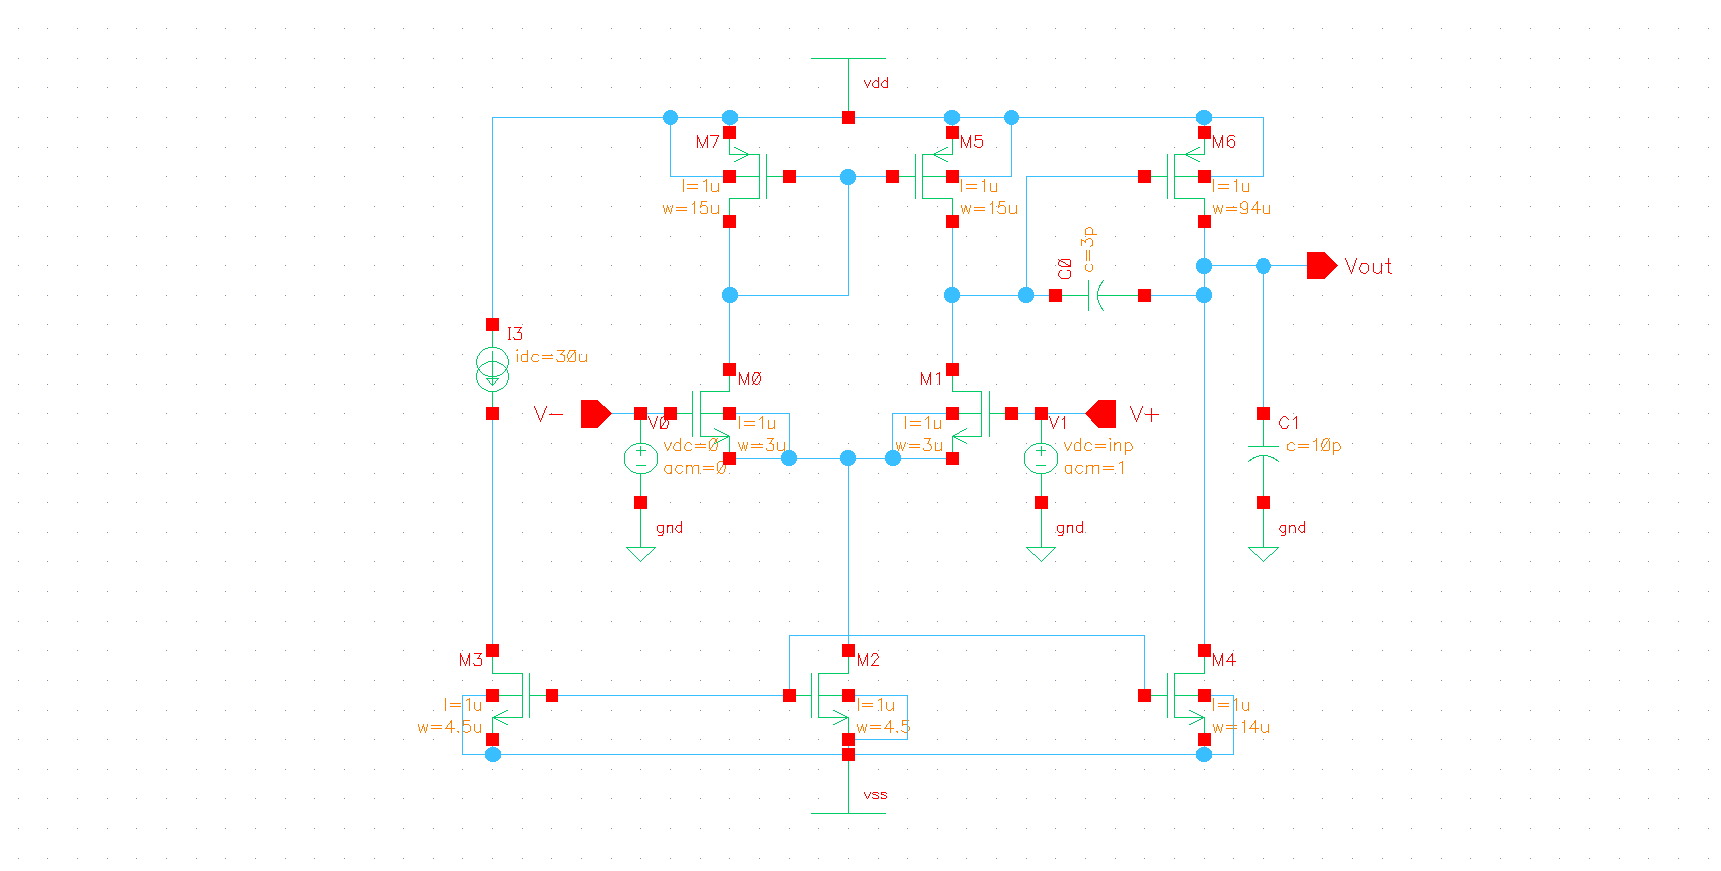
\includegraphics[width=\textwidth]{schematic.png}
    \caption{Schematic diagram of two stage Op-Amp for Transfer Characteristics and Frequency Response.}
    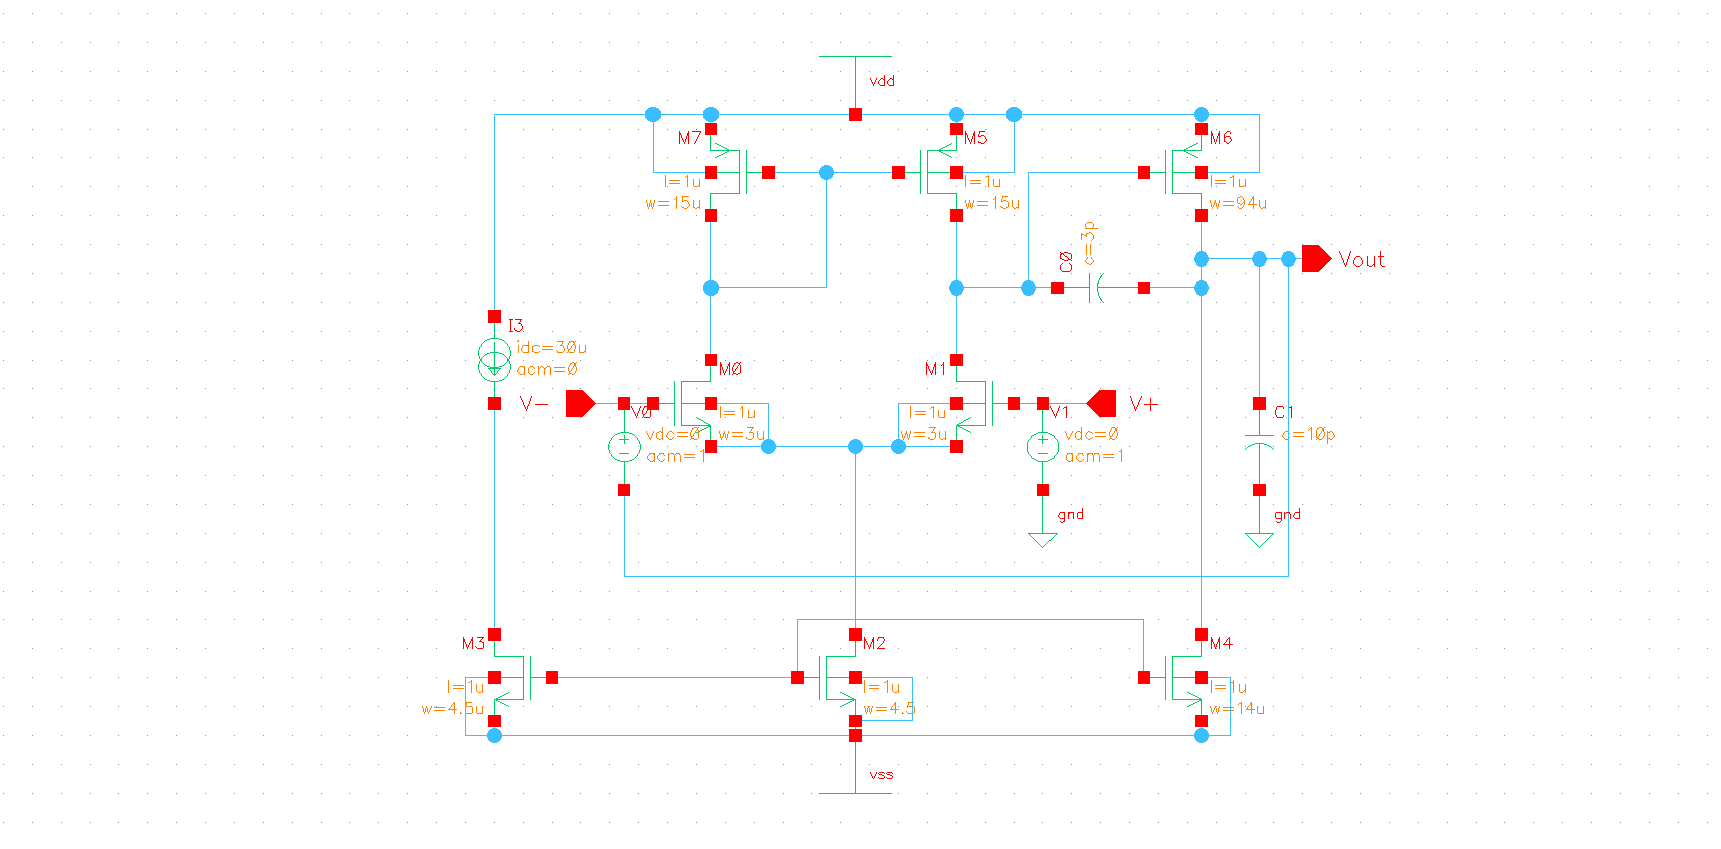
\includegraphics[width=\textwidth]{schematicCMRR.png}
    \caption{Schematic diagram of two stage Op-Amp for CMRR Response.}
    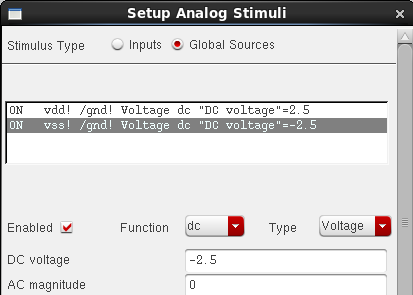
\includegraphics[scale=0.4]{global.png}
    \caption{Global source parameters.}
\end{figure}
\newpage
\section{Simulation Result}
\begin{figure}[!h]
    \centering
    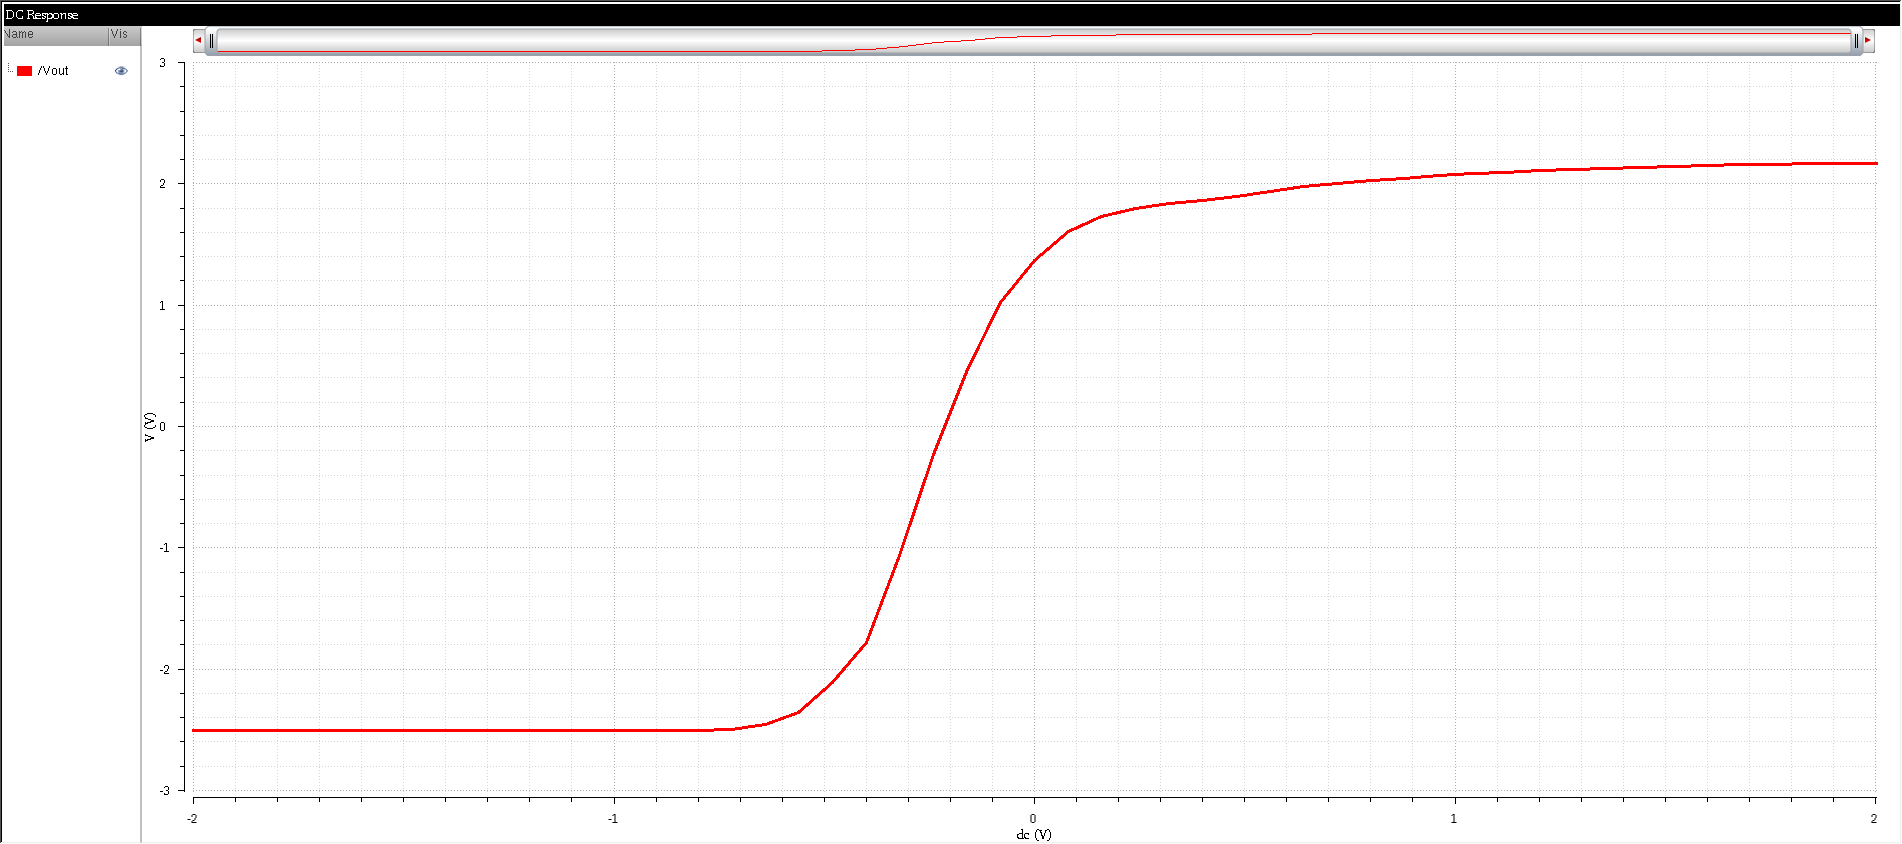
\includegraphics[height=2.8in]{dc.png}
    \caption{Transfer Characteristics of the Op-Amp.}
    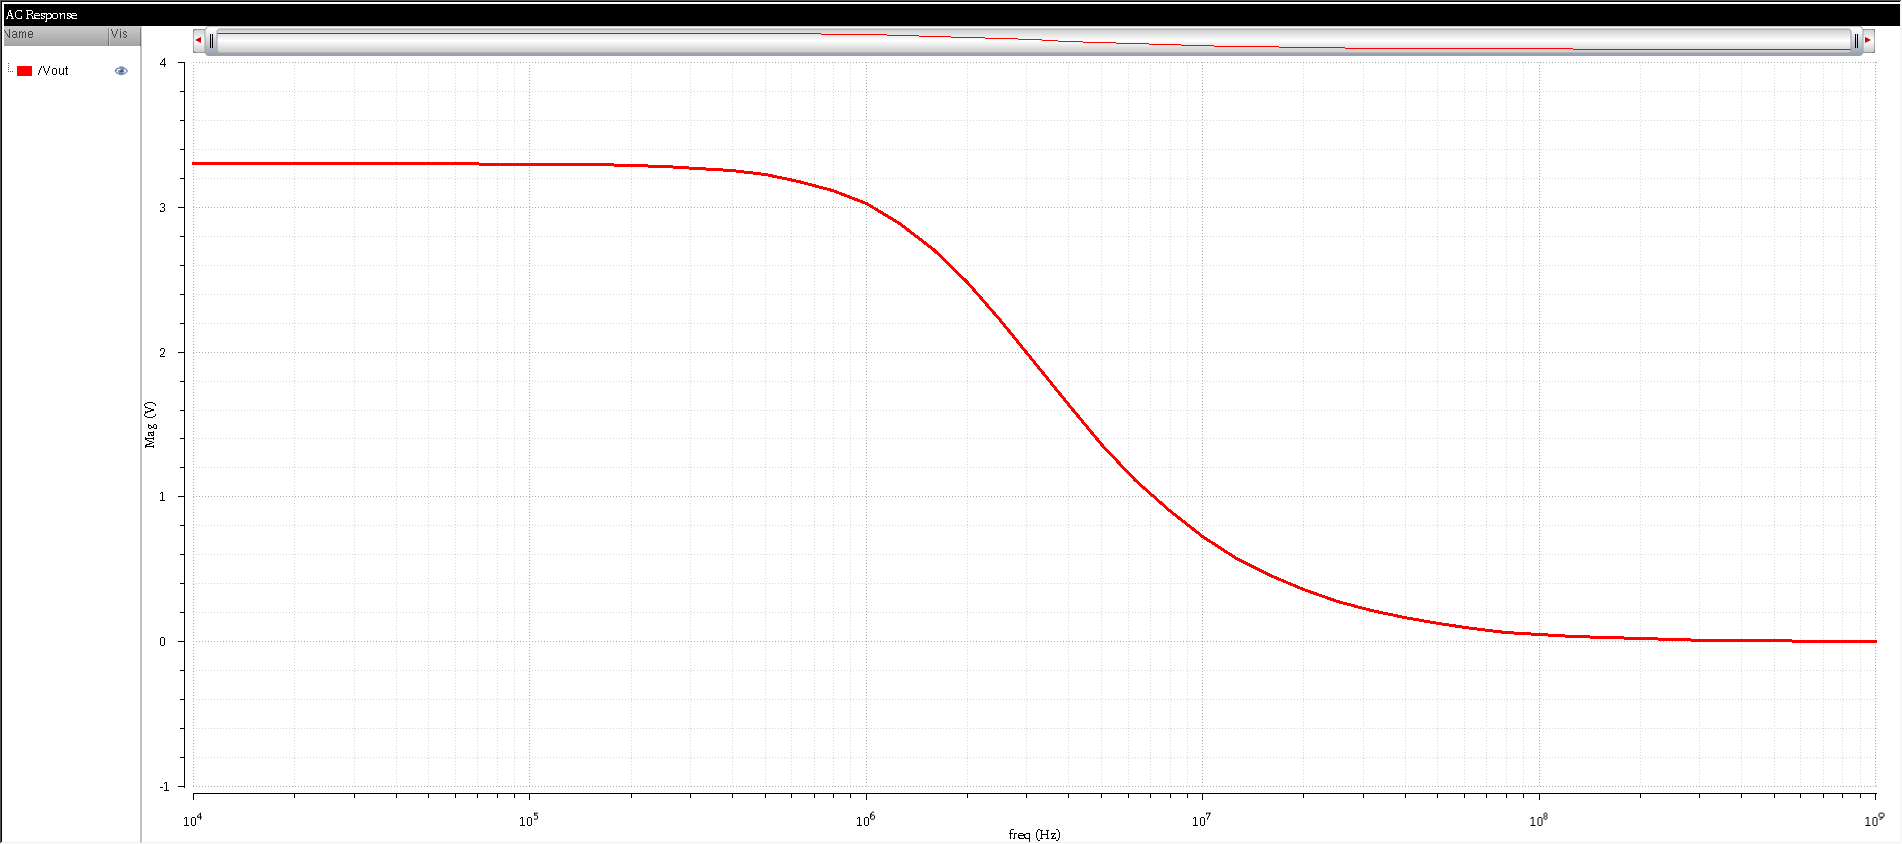
\includegraphics[height=2.8in]{ac.png}
    \caption{Frequency Response of the Op-Amp.}
    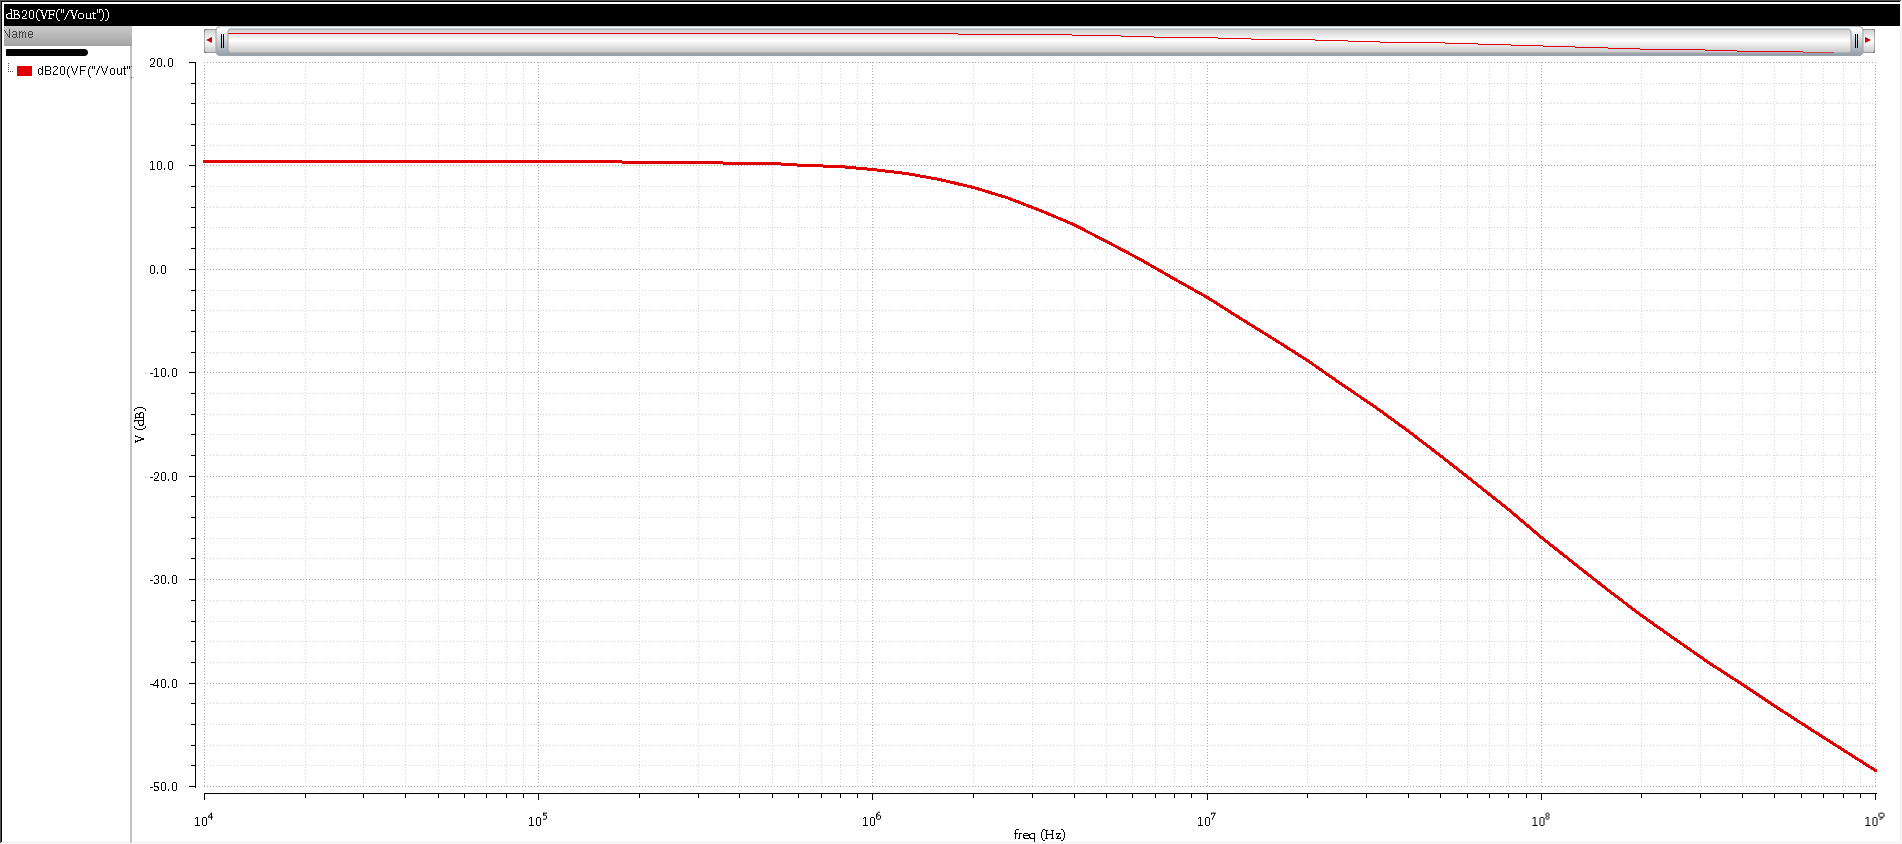
\includegraphics[height=2.8in]{db.png}
    \caption{Frequency Response of the Op-Amp in Decibel(dB) scale.}
\end{figure}
\newpage
\begin{figure}[!h]
    \centering
    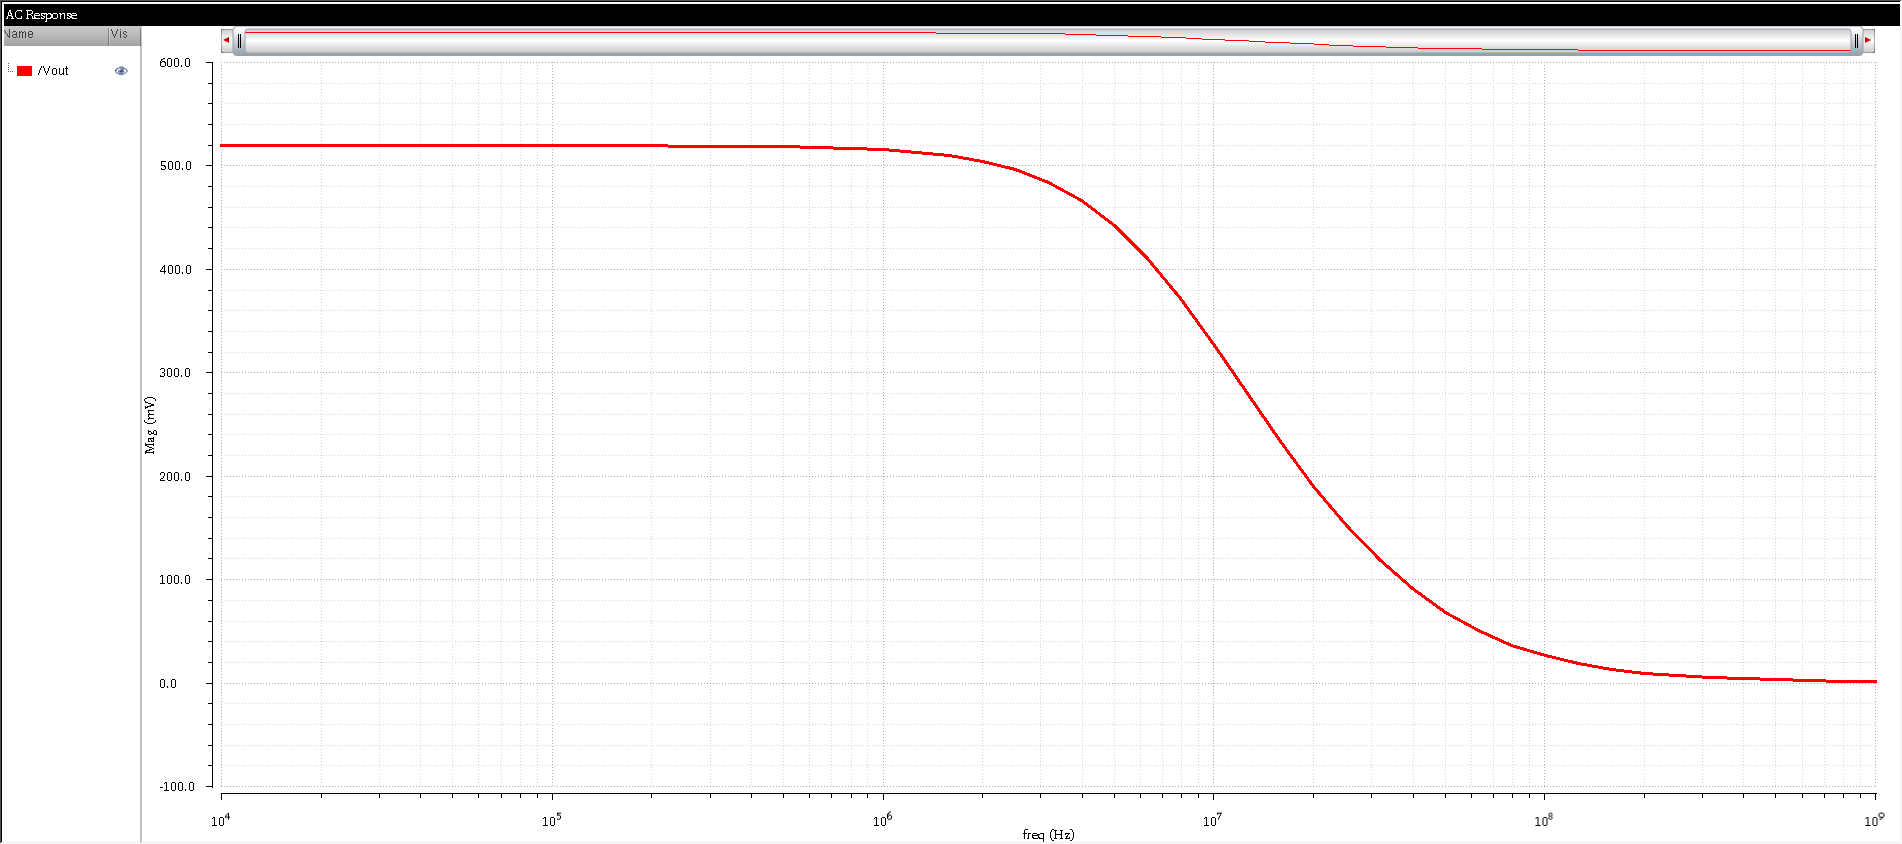
\includegraphics[height=2.8in]{1cmrr.png}
    \caption{Frequency Response of CMRR of the Op-Amp.}
    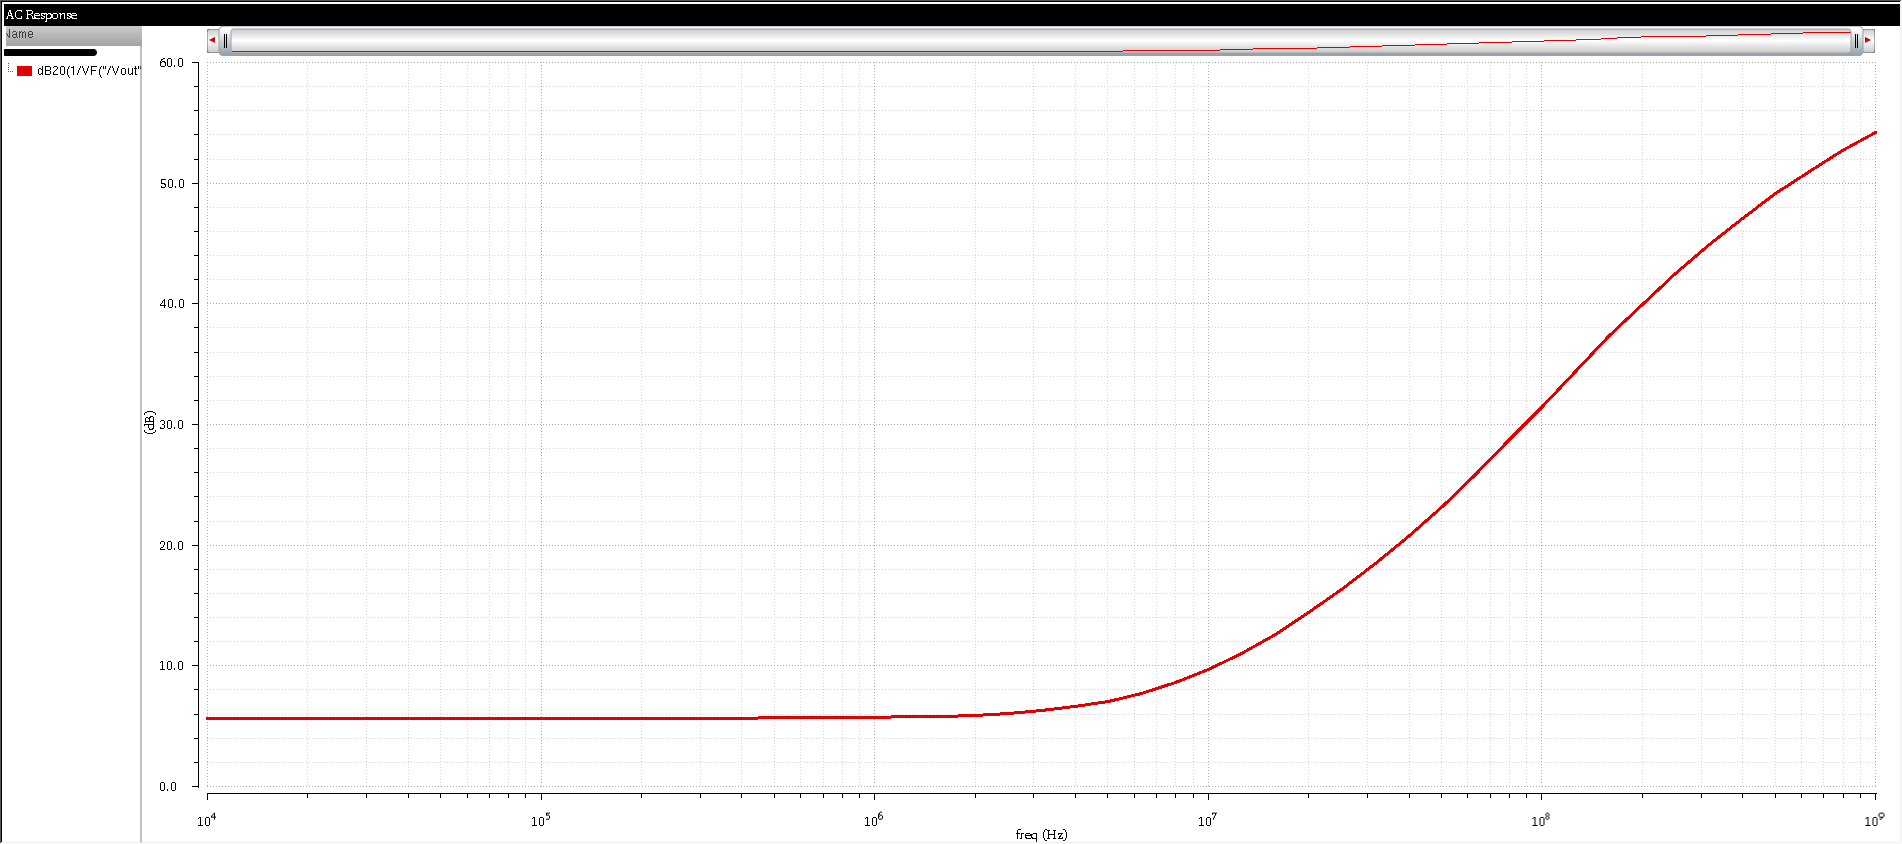
\includegraphics[height=2.8in]{cmrr.png}
    \caption{Frequency Response of (1/CMRR) of the Op-Amp in Decibel(dB) scale.}
\end{figure}
\begin{table}[h!]
    \centering
    \begin{tabular}{|c|c|}
        \hline
        Gain Bandwidth Product (gainBWProd) & $7.541\times10^{6}$ Hz \\
        \hline
        Phase Margin                        & $97.86^\circ$          \\
        \hline
        Gain Margin                         & $-24.34$ dB            \\
        \hline
    \end{tabular}
    \caption{Gain Bandwidth Product, Phase Margin and Gain Margin of the Op-Amp}
\end{table}
\section{Conclusion}
The two-stage CMOS Op-Amp was successfully designed and analyzed using Cadence Virtuoso. The simulations demonstrated compliance with the design specifications in terms of voltage gain, bandwidth, and phase margin. The DC transfer characteristics and frequency response were studied, and the amplifier's Common Mode Rejection Ratio (CMRR) was evaluated. Although corner analysis and Power Supply Rejection Ratio (PSRR) simulations were not performed, the overall results indicate that the Op-Amp meets the required specifications and functions reliably under typical conditions.
\section{References}
\begin{enumerate}
    \item Lab Manual.
    \item Cadence Virtuoso Tutorial - University of Southern California.
\end{enumerate}
\end{document}